\section{Robust Generalization and Flat Minima}
\label{sec:main}

\begin{figure}[t]
	\centering
	\vspace*{-0.2cm}
	\hspace*{-0.4cm}
	\begin{minipage}[t]{0.16\textwidth}
		\vspace*{0px}
		\centering
		\scriptsize 
		\begin{tabularx}{1\textwidth}{|@{\hspace*{1px}}X@{\hspace*{1px}}|@{\hspace*{1px}}c@{\hspace*{1px}}|}
			\hline
			\textbf{Model} & \RTE $\downarrow$\\
			\hline
			\hline
			AT (baseline) {\color{plot0}$\bullet$} & 62.8\\
			Scaled $\times0.5$ {\color{plot1}$\bullet$} & 62.8\\
			Scaled $\times2$ {\color{plot2}$\bullet$} & 62.8\\
			MiSH {\color{plot5}$\bullet$} & 59.8\\
			Batch size $8$ {\color{plot3}$\bullet$} & 58.2\\
			Adam {\color{plot4}$\bullet$} & 57.5\\
			\hline
			\hline
			Label smoothing {\color{plot1}$\bullet$} & 61.2\\
			MART {\color{plot5}$\bullet$} & 61\\
			Entropy-SGD {\color{plot3}$\bullet$} & 58.6\\
			Self-supervision {\color{plot2}$\bullet$} & 57.1\\
			TRADES {\color{plot4}$\bullet$} & 56.7\\
			AT-AWP {\color{plot6}$\bullet$} & 54.3\\
			\hline
		\end{tabularx}
	\end{minipage}
	\begin{minipage}[t]{0.29\textwidth}
		\vspace*{7px}
		
		\begin{minipage}[t]{0.625\textwidth}
			\vspace*{0px}
			
			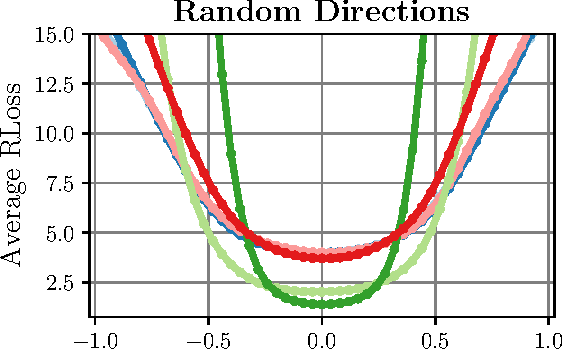
\includegraphics[height=1.85cm]{plots_main_random}
		\end{minipage}
		\begin{minipage}[t]{0.3\textwidth}
			\vspace*{0px}
			
			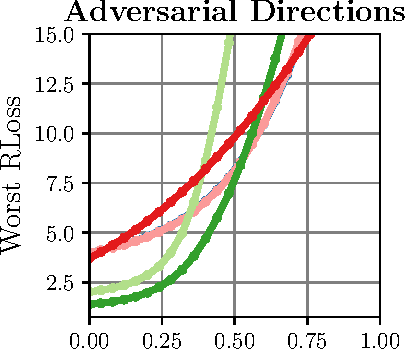
\includegraphics[height=1.85cm]{plots_main_adversarial}
		\end{minipage}
		
		{\rule{5.5cm}{0.25px}}
		\\[-9px]
		\begin{minipage}[t]{0.625\textwidth}
			\vspace*{0px}
			
			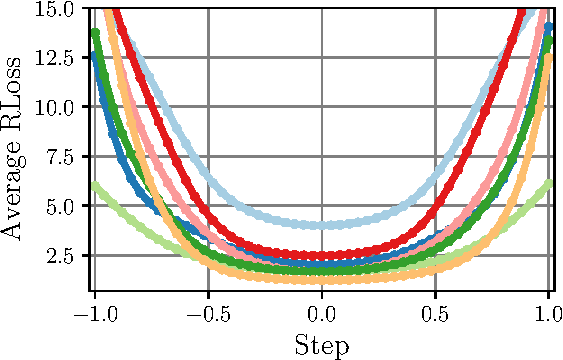
\includegraphics[height=1.9cm]{plots_main_random2}
		\end{minipage}
		\begin{minipage}[t]{0.3\textwidth}
			\vspace*{0px}
			
			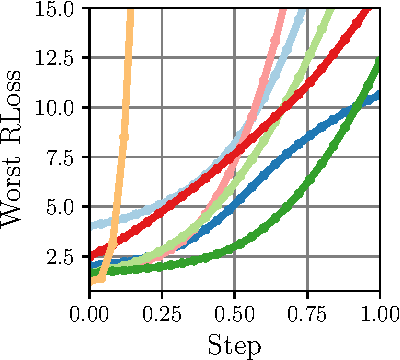
\includegraphics[height=1.9cm]{plots_main_adversarial2}
		\end{minipage}
	\end{minipage}
	
	\vspace*{-10px}
	\caption{\textbf{Visualizing Flatness:} \RCE landscape across $10$ random or adversarial directions. \textbf{Top:} Our AT baseline (ResNet-18) and scaled variants ($\times2$ and $\times0.5$). Training with smaller batch size or Adam \cite{KingmaICLR2015} improves adversarial robustness (lower \RTE vs\onedot AutoAttack \cite{CroceICML2020}) but does \emph{not} result in \emph{visually} flatter minima. \textbf{Bottom:} AT-AWP \cite{WuNIPS2020} or Entropy-SGD \cite{ChaudhariICLR2017} improve robustness \emph{and} visual flatness in random directions. In adversarial directions, however, AT-AWP looks very sharp. Overall, visual inspection does \emph{not} provide a clear, objective picture of flatness.}
	\label{fig:main}
	\vspace*{-6px}
\end{figure}
\begin{figure*}[t]
	\centering
	\vspace*{-0.2cm}
	\begin{minipage}[t]{0.2\textwidth}
		\vspace*{0px}
		
		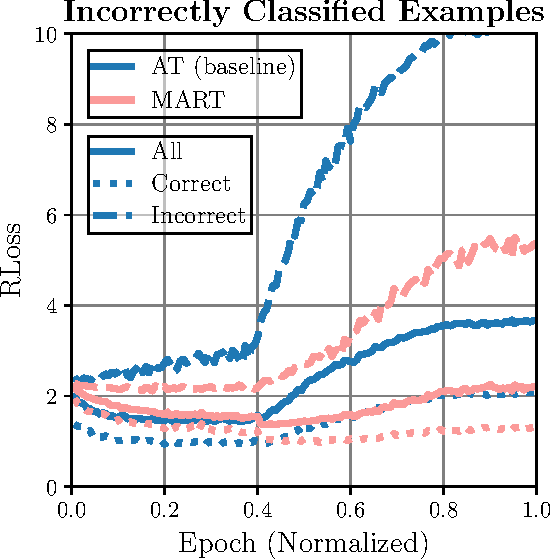
\includegraphics[width=\textwidth]{plots_main_understanding_incorrect2}
	\end{minipage}
	\hspace*{1px}
	\begin{minipage}[t]{0.175\textwidth}
		\vspace*{0px}
		
		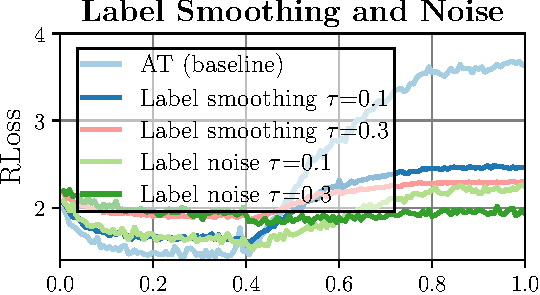
\includegraphics[width=\textwidth]{plots_main_understanding_ls_loss}
		\vspace*{-9px}
		
		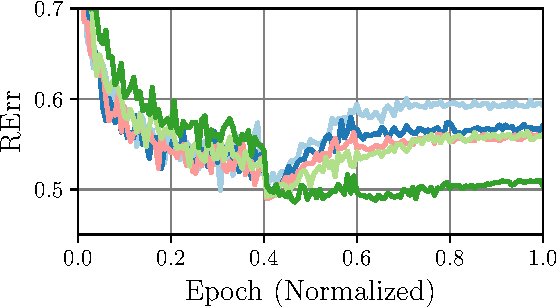
\includegraphics[width=\textwidth]{plots_main_understanding_ls_error}
	\end{minipage}
	\hspace*{1px} 
	\begin{minipage}[t]{0.2\textwidth}
		\vspace*{0px}
		 
		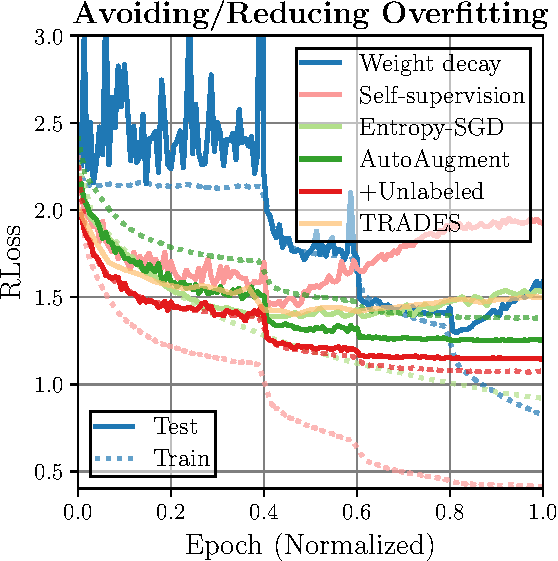
\includegraphics[width=\textwidth]{plots_main_understanding_delay+avoid}
	\end{minipage}
	\hspace*{1px}
	\begin{minipage}[t]{0.175\textwidth}
		\vspace*{0px}
		
		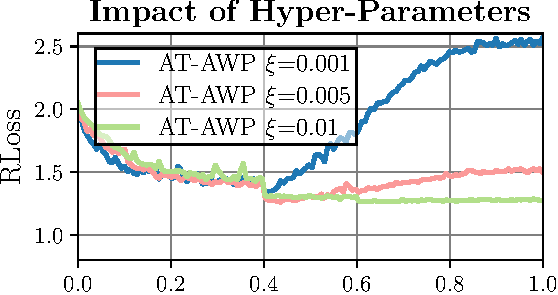
\includegraphics[width=1.025\textwidth]{plots_main_understanding_ablation}
		\vspace*{-9px}
				
		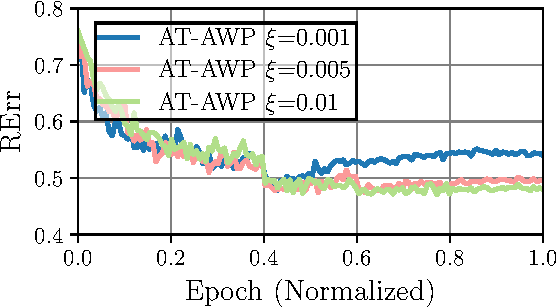
\includegraphics[width=\textwidth]{plots_main_understanding_ablation_error}
	\end{minipage}
	\hspace*{1px}
	\begin{minipage}[t]{0.2\textwidth}
		\vspace*{0px}
	
		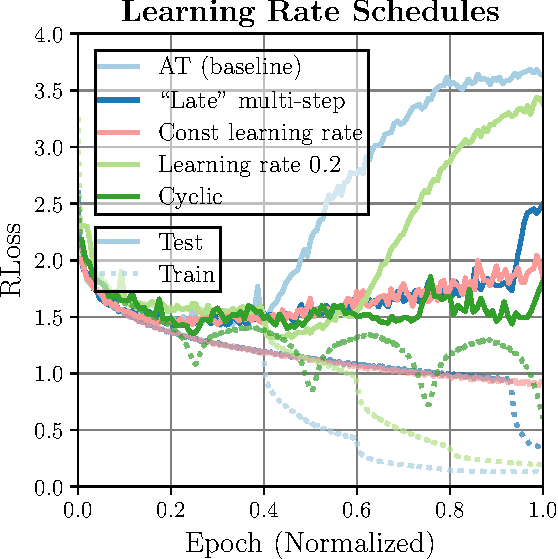
\includegraphics[width=\textwidth]{plots_main_understanding_lr}
	\end{minipage}
	\vspace*{-6px}
	\caption{\textbf{Understanding Robust Overfitting:} Training curves plotted over (normalized) epochs, \red{see \secref{subsec:main-discussion} for detailed discussion}. \textbf{First column:} \RCE, split for correct/incorrect test examples, for AT and MART, which successfully dampens the effect of overfitting using a weighted loss on incorrectly classified examples. \textbf{Second column:} Both label smoothing and label noise reduce robust overfitting \wrt \RCE. However, the reduction in \RCE does not translate to a similar reduction of \RTE. \textbf{Third to fifth column:} \RCE (test solid and train dotted) for various approaches improving adversarial robustness and different learning rate schedules. While some approaches avoid robust overfitting altogether (\eg, AT-AWP), others (\eg, weight decay) merely reduce its impact (third column). But the success depends strongly on hyper-parameters (fourth column). Robust overfitting occurs using all tested learning rate schedules (fifth column), confirming \cite{RiceICML2020}.}
	\label{fig:experiments-understanding}
	\vspace*{-6px}
\end{figure*}

We study robust generalization and overfitting in the context of flatness of the \emph{robust} loss landscape in weight space, \ie, \wrt changes in the weights. While flat minima have consistently been linked to standard generalization \cite{HochreiterNC1997,LiNIPS2018,NeyshaburNIPS2017,KeskarICLR2017}, this relationship remains unclear for adversarial robustness.
We start by briefly introducing the robust overfitting phenomenon (\secref{subsec:main-overfitting}). Then, we discuss problems in judging flatness visually \cite{LiNIPS2018} (\secref{subsec:main-visualization}). Thus, we are inspired by \cite{KeskarICLR2017,NeyshaburNIPS2017} and introduce average- and worst-case flatness measures based on the change in robust loss along random or adversarial weight directions in a local neighborhood (\secref{subsec:main-flatness}), \cf \figref{fig:main-illustration}.
We also discuss the connection of flatness to the Hessian eigenspectrum \cite{YaoNIPS2018} and the importance of scale-invariance as in \cite{DinhICML2017}.

\subsection{Background}
\label{subsec:main-overfitting}

\textbf{Adversarial Training (AT):}
%
Let $f$ be a (deep) neural network taking input $x \in [0,1]^D$ and weights $w \in \mathbb{R}^W$ and predicting a label $f(x;w)$. Given a true label $y$, an adversarial example is a perturbation $\tilde{x} = x + \delta$ such that $f(\tilde{x};w) \neq y$. The perturbation $\delta$ is intended to be nearly invisible which is, in practice, enforced using a $L_p$ constraint: $\|\delta\|_p \leq \epsilon$. To obtain robustness against these perturbations, AT injects adversarial examples during training:
\begin{align}
	\min_w \mathbb{E}_{x,y}\left[\max_{\|\delta\|_p \leq \epsilon} \mathcal{L}(f(x + \delta;w), y)\right]
\end{align}
where $\mathcal{L}$ denotes the cross-entropy loss. The outer minimization problem can be solved using regular stochastic gradient descent (SGD) on mini-batches. To compute adversarial examples, the inner maximization problem is tackled using projected gradient descent (PGD) \cite{MadryICLR2018}. Here, we focus on $p = \infty$ as this constrains the maximum change per feature/pixel, \eg, $\epsilon = \nicefrac{8}{255}$ on \CifarT. For evaluation (at test time), we consider both robust loss (\RCE) $\max_{\|\delta\|_\infty \leq \epsilon} \mathcal{L}(f(x + \delta;w), y)$, approximated using PGD, and robust test error (\RTE), which we approximate using AutoAttack \cite{CroceICML2020}. Note that AutoAttack \red{stops when adversarial examples are found} and does \emph{not} maximize cross-entropy loss, rendering it unfit to estimate \RCE.

\textbf{Robust Overfitting:}
%
Following \cite{RiceICML2020}, \figref{fig:main-overfitting} illustrates the problem of \emph{robust} overfitting, plotting \RCE (left) and \RTE (right) over epochs, which we normalize by the total number of epochs for clarity. Shortly after the first learning rate drop (at epoch $60$, \ie, $40\%$ of training), test \RCE and \RTE start to increase significantly, while robustness on training examples continues to improve.
Robust overfitting was shown to be independent of the learning rate schedule \cite{RiceICML2020} and, as we show (\secref{subsec:experiments-overfitting}), occurs across various different activation functions as well as many popular AT variants.
In contrast to \cite{RiceICML2020}, mostly focusing on \RTE, \figref{fig:main-overfitting} shows that \RCE overfits more severely, indicating a ``disconnectedness'' between \RCE and \RTE that we consider in detail later. For now, \RCE and \RTE do clearly not move ``in parallel'' and \RCE, reaching values around~$4$, is higher than for a random classifier (which is possible considering \emph{adversarial} examples). This is primarily due to an extremely high \RCE on incorrectly classified test examples (which are ``trivial'' adversarial examples). We emphasize, however, that robust overfitting also occurs on correctly classified test examples.

\subsection{Intuition and Visualizing Flatness}
\label{subsec:main-visualization}

\begin{figure*}[t]
	\centering
	\vspace*{-0.2cm}
	\hspace*{-0.1cm}
	\begin{minipage}[t]{0.29\textwidth}
		\vspace*{0px}
		
		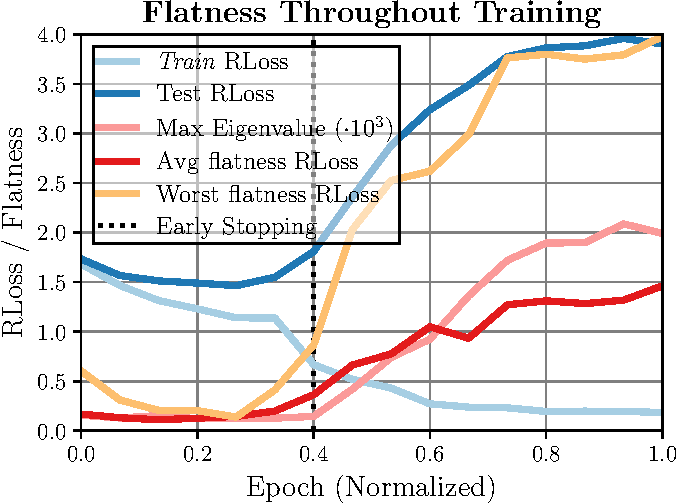
\includegraphics[width=1\textwidth]{plots_main_flatness_epochs}
	\end{minipage}
	\begin{minipage}[t]{0.015\textwidth}
		\vspace*{0px}
		
		\hspace*{4px}{\color{black!75}\rule{0.65px}{3.8cm}}
	\end{minipage}
	\begin{minipage}[t]{0.12\textwidth}
		\vspace*{0px}
		
		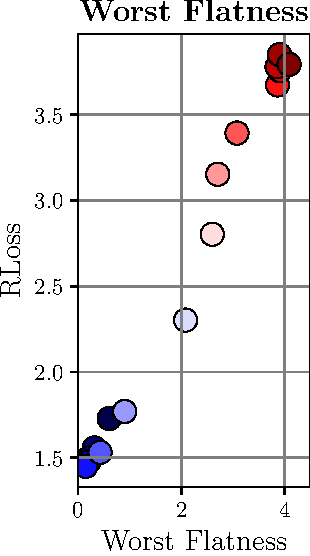
\includegraphics[height=3.7cm]{plots_main_flatness_epochs_correlation_joint}
	\end{minipage}
	\begin{minipage}[t]{0.12\textwidth}
		\vspace*{0px}
		
		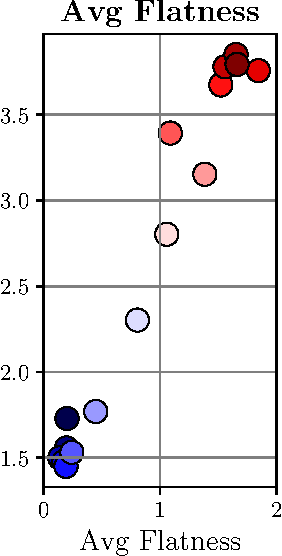
\includegraphics[height=3.7cm]{plots_main_flatness_epochs_correlation_seq}
	\end{minipage}
	\begin{minipage}[t]{0.01\textwidth}
		\vspace*{0px}
		
		\hspace*{4px}{\color{black!75}\rule{0.65px}{3.8cm}}
	\end{minipage}
	\begin{minipage}[t]{0.12\textwidth}
		\vspace*{0px}
		
		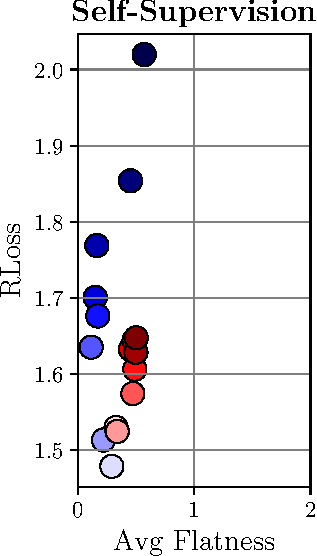
\includegraphics[height=3.7cm]{plots_main_flatness_epochs_correlation_seq_ssl}
	\end{minipage}
	\begin{minipage}[t]{0.112\textwidth}
		\vspace*{0px}
		
		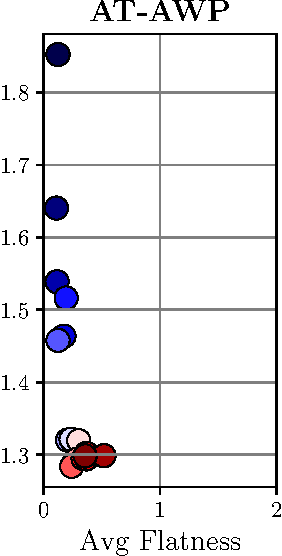
\includegraphics[height=3.7cm]{plots_main_flatness_epochs_correlation_seq_awp}
	\end{minipage}
	\begin{minipage}[t]{0.17\textwidth}
		\vspace*{-2px}
		
		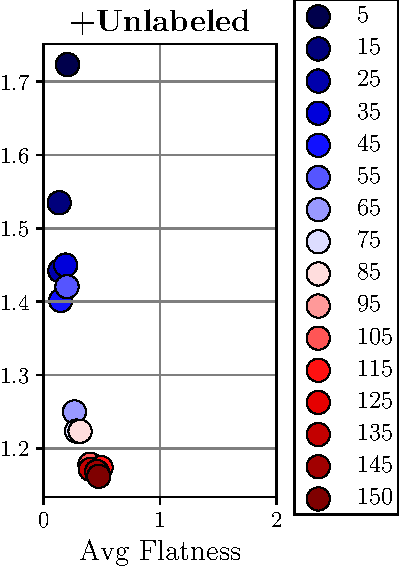
\includegraphics[height=3.7cm]{plots_main_flatness_epochs_correlation_seq_500k}
	\end{minipage}
	\vspace*{-8px}
	\caption{\textbf{Flatness Throughout Training.} \textbf{Left:} Flatness in \RCE throughout training, showing that flatness reduces when the model overfits (\ie, {\color{plot1}test \RCE} increases, while {\color{plot0}train \RCE} decreases). 
	\textbf{Middle:} Test \RCE (y-axis) plotted against flatness in \RCE (x-axis) during training \red{(early epochs in {\color{blue!60!black}dark blue}, late epochs in {\color{red!60!black}dark red})}, showing a clear correlation, for both average- and worst-case flatness.
	\textbf{Right:} AT with self-supervision reduces the impact of robust overfitting (\RCE increases less) and simultaneously favors flatter minima. This behavior is pronounced for AT-AWP, explicitly optimizing flatness, and AT with additional unlabeled examples, generally resulting in the highest adversarial robustness, \cf \tabref{tab:experiments-flatness}.}
	\label{fig:experiments-flatness-epochs}
\end{figure*}

For judging robust flatness, we consider how \RCE changes \wrt random or adversarial perturbations in the weights $w$. Generally, we expect flatter minima to generalize better as the loss does not change significantly within a small neighborhood around the minimum, \ie, the found weights. Then, even if the loss landscape on test examples does not coincide with the loss landscape on training examples, loss remains small, ensuring good generalization. The contrary case, \ie, that sharp minima generalize poorly is illustrated in \figref{fig:main-illustration} (right). Before considering to \emph{measure} flatness, we discuss the easiest way to ``judge'' flatness: visual inspection of the \RCE landscape along random or adversarial directions in weight space.

In \cite{LiNIPS2018}, loss landscape is visualized along \emph{normalized} random directions. Normalization is important to handle different scales, \ie, weight distributions, and allow comparison across models.
We follow \cite{WuNIPS2020} and perform \emph{per-layer} normalization: Letting $\nu \in \mathbb{R}^W$ be a direction in weight space, it is normalized as
%\vskip -2px
\begin{align}
	\hat{\nu}^{(l)} = \frac{\nu^{(l)}}{\|\nu^{(l)}\|_2} \|w^{(l)}\|_2 \quad\text{ for layer }l.\label{eq:main-normalization}
\end{align}
\vskip -2px
In contrast to \cite{LiNIPS2018}, we also consider biases and treat them as individual layer, but we exclude batch normalization parameters.
Then, the loss landscape is visualized in discrete steps along this direction, \ie, $w + s\hat{\nu}$ for $s \in [-1, 1]$.
Adversarial examples are computed ``on-the-fly'', \ie, for each $w + s\hat{\nu}$ individually, to avoid underestimating \RCE as in \cite{YuARXIV2018,PrabhuARXIV2019}.
The result is indeed scale-invariant: \figref{fig:main} (top) shows that the loss landscapes for scaled versions (factors $0.5$ or $2$, see supplementary material) of our AT baseline coincide with the original landscape.
However, \figref{fig:main} also illustrates that judging flatness visually is difficult: Considering random weight directions, AT with Adam \cite{KingmaICLR2015} or small batch size improves adversarial robustness, but the found minima look less flat (top). For other approaches, \eg, TRADES \cite{ZhangICML2019} or AT-AWP \cite{WuNIPS2020}, results look indeed flatter while also improving robustness (bottom). In adversarial directions, in contrast, AT-AWP looks particularly sharp. Furthermore, not only flatness but also the vertical ``height'' of the loss landscape matters and it is impossible to tell ``how much'' flatness is necessary.

\subsection{Average- and Worst-Case Flatness Measures}
\label{subsec:main-flatness}

In order to objectively measure and compare flatness, we draw inspiration from \cite{NeyshaburNIPS2017,KeskarICLR2017} and propose average- and worst-case flatness measures adapted to the robust loss. \red{We emphasize that measuring flatness in \RCE is non-trivial and flatness in (clean) \CE \emph{cannot} be expected to correlate with robustness (see supplementary material). For example, we need to ensure scale-invariance \cite{DinhICML2017} and estimate \RCE \emph{on top} of random or adversarial weight perturbations:}

\textbf{Average-Case / Random Flatness:}
%
Considering random weight perturbations $\nu \in B_\xi(w)$ within the $\xi$-neighborhood of $w$, average-case flatness is computed as
\vspace*{-12px}
\begin{align}
	\hspace*{-8px}
	\begin{split}
		\mathbb{E}_{\nu}[\max\limits_{\|\delta\|_\infty \leq \epsilon} \mathcal{L}(f(x{+}\delta; w{+}\nu), y)]\text{\hphantom{aaaaaaaaaaa}}\\[-2px]
		\text{\hphantom{aaaaaaaaaaa}}- \max\limits_{\|\delta\|_\infty \leq \epsilon} \mathcal{L}(f(x{+}\delta;w), y)
	\end{split}\label{eq:main-average}
\end{align}
\vskip -4px
\noindent averaged over test examples $x,y$, as illustrated in \figref{fig:main-illustration}. We define $B_\xi(w)$ using \emph{relative} $L_2$-balls per layer (\cf \eqnref{eq:main-normalization}): 
%\vskip -2px
\begin{align}
	B_\xi(w) = \{w + \nu : \|\nu^{(l)}\|_2 \leq \xi \|w^{(l)}\|_2 \forall\text{ layers }l\}.\label{eq:main-ball}
\end{align}
\vskip -2px
\red{This ensures scale-invariance \wrt the weights as $B_\xi(w)$ scales with the weights on a \emph{per-layer} basis.}
Note that the second term in \eqnref{eq:main-average}, \ie, the ``reference'' robust loss, is important to make the measure independent of the absolute loss (\ie, corresponding to the vertical shift in \figref{fig:main}, left).
In practice, $\xi$ can be as large as $0.5$. We refer to \eqnref{eq:main-average} as \textbf{average-case flatness in \RCE}.

\textbf{Worst-Case / Adversarial Flatness:} \cite{WuNIPS2020} explicitly optimizes flatness in \emph{adversarial weight} directions and shows that average-case flatness is not sufficient to improve adversarial robustness. As it is unclear whether \cite{WuNIPS2020} actually improves worst-case flatness, we define
%\vskip -2px
\begin{align}
	\begin{split}
		\max\limits_{\nu \in B_\xi(w)}&\left[\max\limits_{\|\delta\|_\infty \leq \epsilon} \mathcal{L}(f(x{+}\delta; w{+}\nu), y)\right]\hphantom{aaaaaa}\\[1px]
		&\hphantom{aaaaaaaa}- \max\limits_{\|\delta\|_\infty \leq \epsilon} \mathcal{L}(f(x{+}\delta;w), y)
	\end{split}\label{eq:main-worst}
\end{align}
\vskip -2px
as \textbf{worst-case flatness in \RCE}. Here, we use the same definition of $B_\xi(w)$ as above (aligned with \cite{WuNIPS2020}), but for smaller values of $\xi$.
Regarding \emph{standard} performance, this worst-case notion of flatness has been shown to be a reliable predictor of generalization \cite{JiangICLR2020,KeskarICLR2017}. For computing \eqnref{eq:main-worst} in practice, we jointly optimize over $\nu$ and $\delta$ (for each batch individually) using PGD.
As illustrated in \figref{fig:main}, \RCE increases quickly along adversarial directions, even for very small values of $\xi$, \eg, $\xi = 0.005$.

\subsection{Discussion}
\label{subsec:main-discussion}

In the context of flatness, there has also been some discussion concerning the meaning of Hessian eigenvalues \cite{LiNIPS2018,YaoNIPS2018} as well as concerns regarding the scale-invariance of flatness measures \cite{DinhICML2017}. First, regarding the Hessian eigenspectrum,
\cite{YaoNIPS2018} shows that large Hessian eigenvalues indicate poor adversarial robustness. However, Hessian eigenvalues are generally \emph{not} scale-invariant (which is acknowledged in \cite{YaoNIPS2018}): Our AT baseline has a maximum eigenvalue of $1990$ which reduces to $505$ when \emph{up-scaling} the model and increases to $7936$ when \emph{down-scaling}, without affecting robustness (\cf $\times0.5$ and $\times2$ in \figref{fig:main}). We also found that the largest eigenvalue is \emph{not} correlated with adversarial robustness. Second, following a similar train of thought, \cite{DinhICML2017} criticizes the flatness measures of \cite{NeyshaburNIPS2017,KeskarICLR2017} as not being scale-invariant. That is, through clever scaling of weights, without changing predictions, arbitrary flatness values can be ``produced''. However, the analysis in \cite{DinhICML2017} does not take into account the relative neighborhood as defined in \cite{KeskarICLR2017}, which renders the measure explicitly scale-invariant. This also applies to our definition of $B_\xi(w)$ in \eqnref{eq:main-ball} and is shown in \figref{fig:main} where normalization is performed relative \red{(per-layer)} to the weights; \red{empirical validation can be found in the supplementary material.}

\section{Experiments}
\label{sec:experiments}

We start with a closer look at \RCE in robust overfitting (\secref{subsec:experiments-overfitting}, \figref{fig:experiments-understanding}). Then, we show a strong correlation between good robust generalization and flatness (\secref{subsec:experiments-flatness}). \red{For example, robust overfitting causes sharper minima (\figref{fig:experiments-flatness-epochs}). More importantly, more robust models generally find flatter minima and, vice-versa, methods encouraging flatness improve adversarial robustness (\figref{fig:experiments-flatness-methods}, \ref{fig:experiments-flatness-correlation}).} In fact, flatness improves robust generalization by \emph{both} lowering the robust generalization gap \red{(incl. a reduction in robust overfitting, \cf \figref{fig:experiments-flatness-gap})}.

\begin{figure}[t]
	\centering
	\vspace*{-0.2cm}
	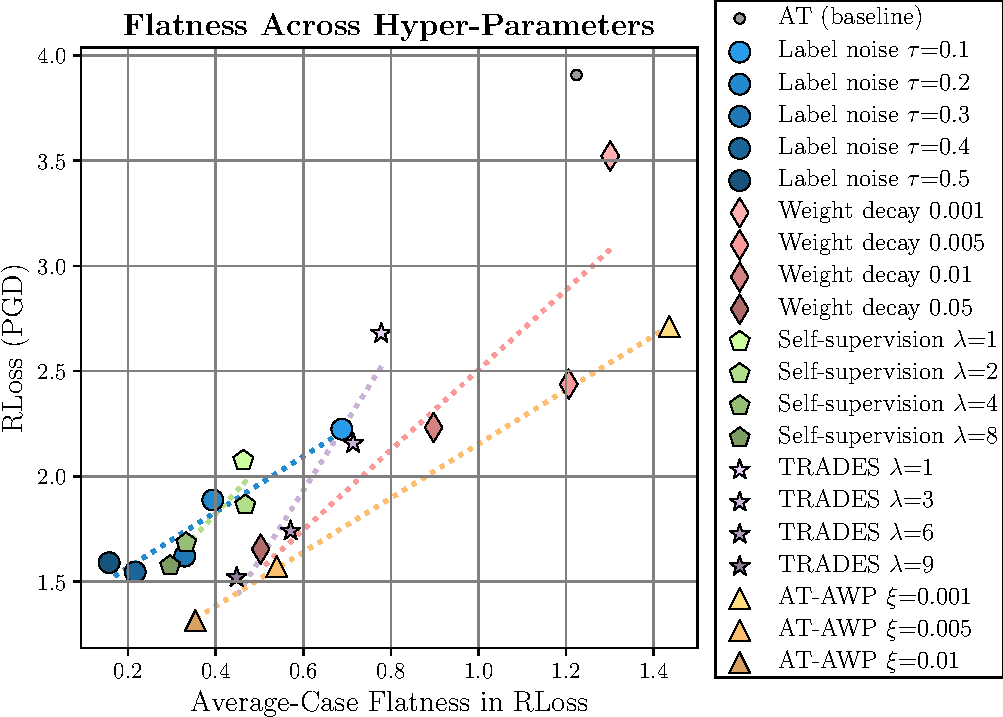
\includegraphics[width=0.4\textwidth]{plots_main_flatness_methods}
	\vspace*{-6px}
	\caption{\textbf{Flatness Across Hyper-Parameters:} \RCE (y-axis) vs\onedot average-case flatness (x-axis) for selected methods and hyper-parameters (\cf supplementary material). For example, we consider different strengths of weight decay ({\color{plot2}rose}) or sizes $\xi$ of adversarial weight perturbations for AT-AWP ({\color{plot10!80!black}orange}). For clarity, we plot (dotted) lines representing the trend per method. Clearly, improved adversarial robustness, \ie, low \RCE, is related to improved flatness.}
	\label{fig:experiments-flatness-methods}
	\vspace*{-6px}
\end{figure}

\textbf{Setup:} 
%
On \CifarT \cite{Krizhevsky2009}, our \emph{AT baseline} uses ResNet-18 \cite{HeCVPR2016} and is trained for $150$ epochs, batch size $128$, learning rate $0.05$, reduced by factor $0.1$ at $60$, $90$ and $120$ epochs, using weight decay $0.005$ and momentum $0.9$ with standard SGD. We use random flips and cropping as data augmentation. During training, we use $7$ iterations PGD, with learning rate $0.007$, signed gradient and $\epsilon = \nicefrac{8}{255}$ for $L_\infty$ adversarial examples. PGD-$7$ is also used for early stopping (every $5$th epoch) on the last $500$ test examples. We do \emph{not} use early stopping by default. For evaluation on the first $1000$ test examples, we run PGD with $20$ iterations, $10$ random restarts to estimate \RCE and AutoAttack \cite{CroceICML2020} to estimate \RTE\xspace\red{(\cf \secref{subsec:main-overfitting})}. For \emph{average-case flatness of \RCE}, we \red{take the average of} $10$ random weight perturbations with $\xi{=}0.5$. For \emph{worst-case flatness}, we maximize \RCE jointly over adversarial examples and adversarial weights with $\xi{=}0.00075$, \red{taking the worst of $10$ restarts.}
 
\textbf{Methods:}
%
Besides our AT baseline, we consider AT-AWP \cite{WuNIPS2016}, TRADES \cite{ZhangICML2019}, MART \cite{WangICLR2020}, AT with self-supervision \cite{HendrycksNIPS2019} or additional unlabeled examples \cite{CarmonNIPS2019,UesatoNIPS2019}, weight averaging \cite{IzmailovUAI2018} and AT with ``early-stopped'' PGD \cite{ZhangICML2020}. We investigate different hyper-parameters and ``tricks'' recently studied in \cite{PangARXIV2020b,GowalARXIV2020}: learning rate schedules, batch size, weight decay, label smoothing \cite{SzegedyCVPR2016} as well as SiLU/Mish/GeLU \cite{ElfwingNN2018,MisraBMVC2020,HendrycksARXIV2016} activation functions. Furthermore, we consider Entropy-SGD \cite{ChaudhariICLR2017}, label noise, weight clipping \cite{StutzMLSYS2021} and AutoAugment \cite{CubukARXIV2018}. We emphasize that weight averaging, Entropy-SGD and weight clipping are known to improve flatness of the (clean) loss.
\red{\emph{If not stated otherwise, these methods are applied on top or as replacement of our AT baseline.}}
We report results using the best hyper-parameters per method. Finally, we also use pre-trained models from RobustBench \cite{CroceARXIV2020b}, which were obtained using early stopping. 

\begin{table}[t]
	\centering
	\vspace*{-0.25cm}
	\hspace*{-0.4cm}
	{
	\scriptsize
	\setlength{\tabcolsep}{0pt}
    \newcolumntype{C}[1]{@{}>{\centering\arraybackslash}p{#1}@{}}
	\begin{tabularx}{0.5\textwidth}{|X|C{0.85cm}|C{1.4cm}|C{0.85cm}|C{0.85cm}||C{1.4cm}|}
		\hline
		\hspace*{2px} \bfseries Model & \multicolumn{2}{c|}{\bfseries Robustness $\downarrow$} & \multicolumn{2}{c||}{\bfseries Flatness $\downarrow$} & \bfseries Early Stop.\\
		\hline
		\hspace*{2px}\textcolor{colorbrewer1}{(sorted asc. by test \RTE)} & \RTE & \RTE & Avg & Worst & \RTE $\downarrow$\\
		\hspace*{2px}\textcolor{gray}{(split at $70\%$/$30\%$ percentiles)} & (test) & (train) & (\RCE) & (\RCE) & (early stop)\\
		\hline
		\hline		
		\rowcolor{colorbrewer3!15}\hspace*{2px} +Unlabeled & 48.9 & 43.2 (-5.7) & 0.32 & 1.20 & 48.9 (-0.0)\\
		\rowcolor{colorbrewer3!15}\hspace*{2px} Cyclic & 53.6 & 35.4 (-18.2) & 0.35 & 1.50) & 53.6 (-0.0)\\
		\rowcolor{colorbrewer3!15}\hspace*{2px} AutoAugment & 54.0 & 47.9 (-6.1) & 0.49 & 0.69 & 53.5 (-0.5)\\
		\rowcolor{colorbrewer3!15}\hspace*{2px} AT-AWP & 54.3 & 43.1 (-11.2) & 0.35 & 2.68 & 53.6 (-0.7)\\
		\rowcolor{colorbrewer3!15}\hspace*{2px} Label noise & 56.2 & 30.0 (-26.2) & 0.33 & 0.93) & 55.5 (-0.7)\\
		\rowcolor{colorbrewer3!15}\hspace*{2px} Weight clipping & 56.5 & 39.0 (-17.5) & 0.41 & 4.57 & 56.5 (-0.0)\\
		\rowcolor{colorbrewer3!15}\hspace*{2px} TRADES & 56.7 & 15.8 (-40.9) & 0.57 & 2.25 & 53.4 (-3.3)\\
		\hline
		\rowcolor{colorbrewer5!15}\hspace*{2px} Self-supervision & 57.1 & 45.0 (-12.1) & 0.33 & 2.63 & 56.8 (-0.3)\\
		\rowcolor{colorbrewer5!15}\hspace*{2px} Weight decay & 58.1 & 32.8 (-25.3) & 0.50 & 3.93 & 54.8 (-3.3)\\
		\rowcolor{colorbrewer5!15}\hspace*{2px} Entropy-SGD & 58.6 & 46.1 (-12.5) & 0.28 & 1.80 & 56.9 (-1.7)\\
		\rowcolor{colorbrewer5!15}\hspace*{2px} MiSH & 59.8 & 5.3 (-54.5) & 1.56 & 3.54 & 53.7 (-6.1)\\
		\rowcolor{colorbrewer5!15}\hspace*{2px} ``Late'' multi-step & 59.8 & 18.4 (-41.4) & 0.80 & 2.96 & 57.8 (-2.0)\\
		\hline
		\rowcolor{colorbrewer1!15}\hspace*{2px} SiLU & 60.0 & 5.6 (-54.4) & 1.71 & 4.20 & 53.7 (-6.3)\\
		\rowcolor{colorbrewer1!15}\hspace*{2px} Weight averaging & 60.0 & 10.0 (-50.0) & 1.28 & 5.98 & 53.0 (-7.0)\\
		\rowcolor{colorbrewer1!15}\hspace*{2px} Larger $\epsilon{=}\nicefrac{9}{255}$ & 60.9 & 11.1 (-49.8) & 1.33 & 5.84 & 53.8 (-7.1)\\
		\rowcolor{colorbrewer1!15}\hspace*{2px} MART & 61.0 & 20.8 (-40.2) & 0.73 & 3.17 & 54.7 (-6.3)\\
		\rowcolor{colorbrewer1!15}\hspace*{2px} GeLU & 61.1 & 3.2 (-57.9) & 1.55 & 4.12 & 56.7 (-4.4)\\
		\rowcolor{colorbrewer1!15}\hspace*{2px} Label smoothing & 61.2 & 8.0 (-53.2) & 0.65 & 2.72 & 54.0 (-7.2)\\
		\rowcolor{colorbrewer1!15}\hspace*{2px} AT (baseline) & 62.8 & 10.7 (-52.1) & 1.21 & 6.48 & 54.6 (-8.2)\\
		\hline
	\end{tabularx}
	}
	
	\hspace*{-0.38cm}
	{
	\tiny
	\setlength{\tabcolsep}{0pt}
 	\newcolumntype{C}[1]{@{}>{\centering\arraybackslash}p{#1}@{}}
	\begin{tabularx}{0.5\textwidth}{|X|C{0.85cm}|C{1.4cm}|C{0.85cm}|C{0.85cm}||C{1.4cm}|}
		\hline
		\hspace*{2px} \bfseries Robustness & \multicolumn{5}{c|}{\bfseries Averages (across models)}\\
		\hline
		\rowcolor{colorbrewer3!15}\hspace*{2px} Good ($\RTE{<}57\%{\approx}30\%$ percentile) & 54.3 & 36.3 (-18.0) & 0.40 & 2.00 & 53.6 (-0.7)\\
		\rowcolor{colorbrewer5!15}\hspace*{2px} Average ($57\%{\geq}\RTE < 60\%$) & 58.7 & 29.5 (-29.2) & 0.69 & 2.9 & 56.0 (-2.7)\\
		\rowcolor{colorbrewer1!15}\hspace*{2px} Poor ($\RTE{\geq}60\%{\approx}70\%$ percentile) & 61.0 & 9.9 (-51.1) & 1.21 & 4.67 & 54.4 (-6.6)\\
		\hline
	\end{tabularx}
	}
	\vspace*{-6px}
	\caption{\textbf{Robustness and Flatness, Quantitative Results:} Test and train \RTE (first, second column, early stopping in fifth column) as well as average-/worst-case flatness in \RCE (third, fourth column) for selected methods, \cf \figref{fig:experiments-flatness-correlation}.
	We split methods into \colorbox{colorbrewer3!15}{good}, \colorbox{colorbrewer5!15}{average}, and \colorbox{colorbrewer1!15}{poor} robustness using the $30\%$ and $70\%$ percentiles.
	Most methods improve adversarial robustness alongside both average- and worst-case flatness.
	}
	\label{tab:experiments-flatness}
	\vspace*{-6px}
\end{table}
\begin{figure*}[t]
	\centering
	\vspace*{-0.2cm}
	\hspace*{-0.4cm}
	\begin{minipage}[t]{0.29\textwidth}
		\vspace*{0px}
		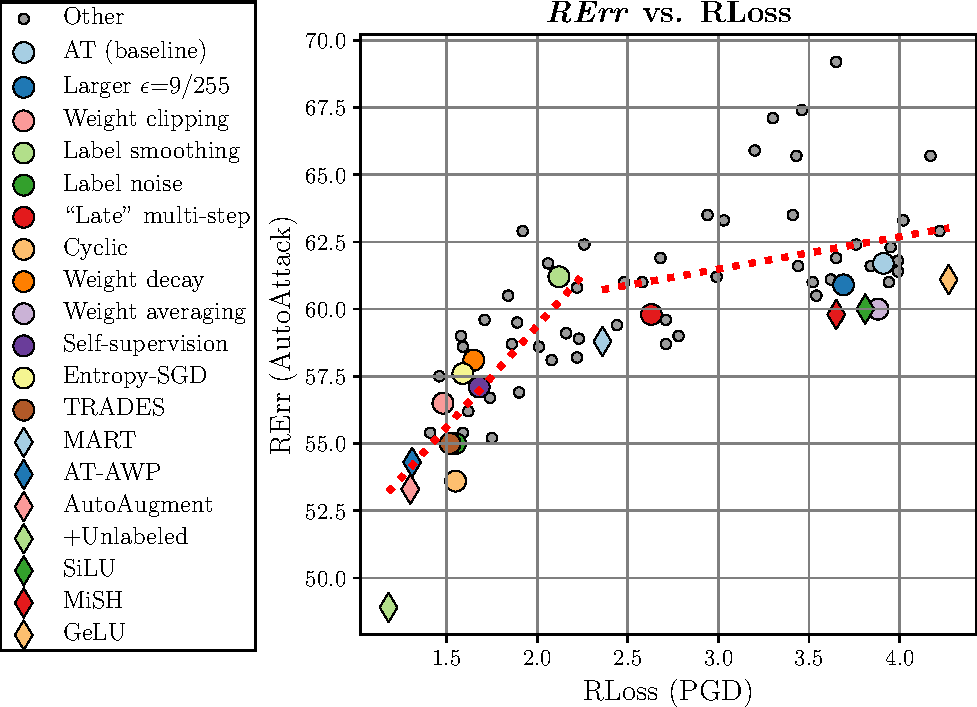
\includegraphics[height=3.8cm]{plots_main_loss_error}
	\end{minipage}
	\hspace*{2px}
	\begin{minipage}[t]{0.01\textwidth}
		\vspace*{0px}
		
		\hspace*{4px}{\color{black!75}\rule{0.65px}{3.8cm}}
	\end{minipage}
	\hspace*{2px}
	\begin{minipage}[t]{0.21\textwidth}
		\vspace*{0px}
		
		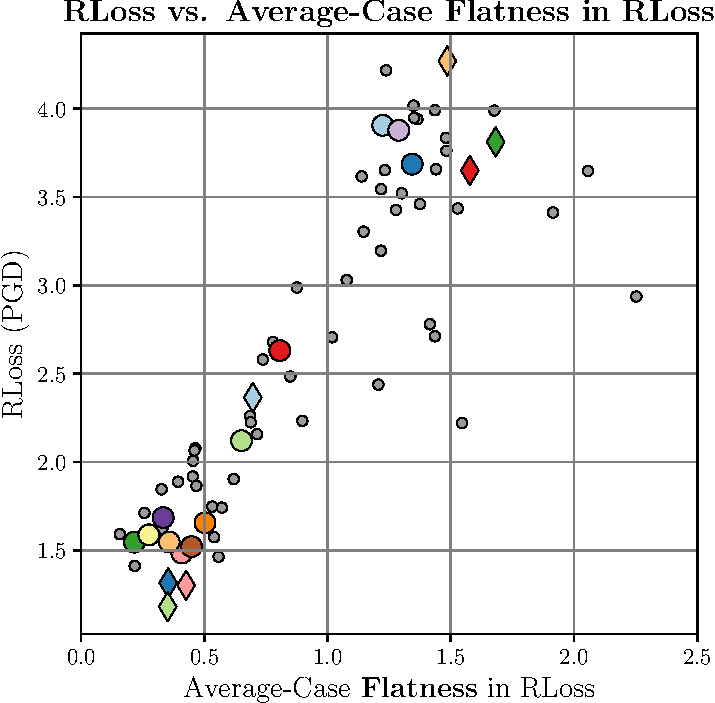
\includegraphics[height=3.8cm]{plots_main_flatness_correlation_seq_loss}
	\end{minipage}
	\hspace*{2px}
	\begin{minipage}[t]{0.21\textwidth}
		\vspace*{0px}
		
		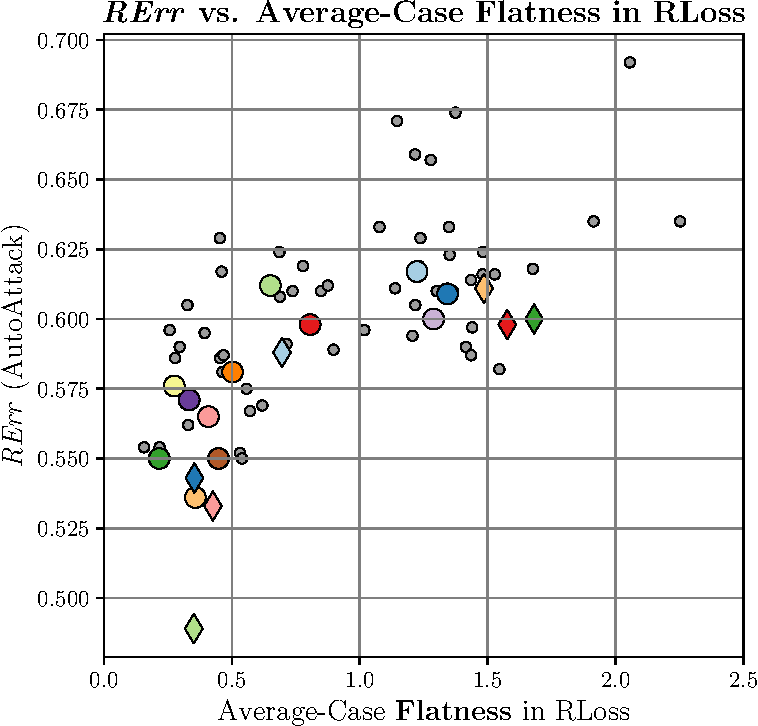
\includegraphics[height=3.8cm]{plots_main_flatness_correlation_seq_error}
	\end{minipage}
	\hspace*{2px}
	\begin{minipage}[t]{0.01\textwidth}
		\vspace*{0px}
		
		\hspace*{4px}{\color{black!75}\rule{0.65px}{3.8cm}}
	\end{minipage}
	\hspace*{2px}
	\begin{minipage}[t]{0.2\textwidth}
		\vspace*{0px}
		
		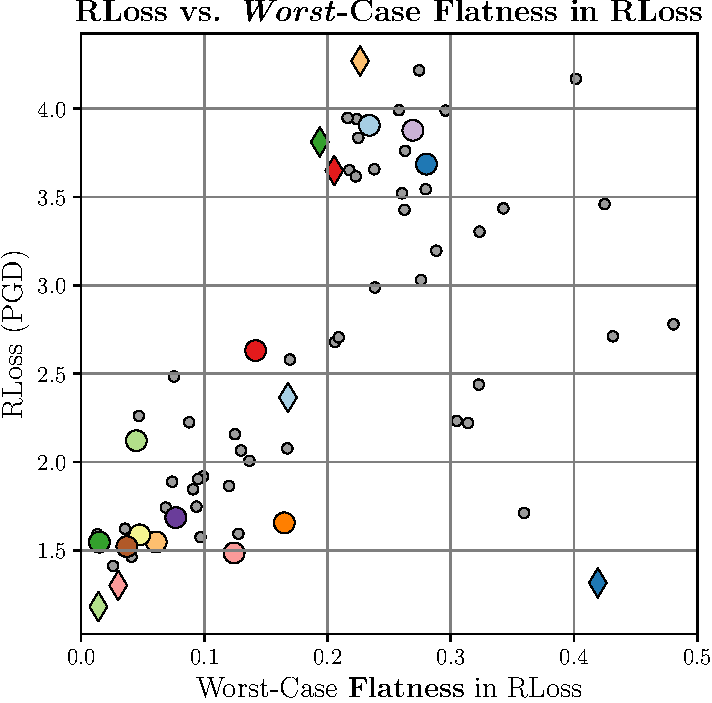
\includegraphics[height=3.8cm]{plots_main_flatness_correlation_joint_loss}
	\end{minipage}
	
	\vspace*{-6px}
	\caption{\textbf{Robustness and Flatness:} \textbf{Left:} \RTE plotted against \RCE, showing that improved \RCE does not directly translate to reduced \RTE for large \RCE. In these cases, reducing \RCE mainly means reducing the confidence of adversarial examples, which is necessary to improve adversarial robustness. \textbf{Middle:} \RCE or \RTE (y-axis) plotted against our \emph{average-case} flatness in \RCE. We highlight selected models, as in \tabref{tab:experiments-flatness}. Considering \RCE, we reveal a striking correlation between adversarial robustness and flatness. Popular AT variants improving robustness (\eg, {\color{plot11}TRADES}, {\color{plot0}MART}, \etc) also correspond to flatter minima. Vice versa, methods improving flatness (\eg, {\color{plot10}Entropy-SGD}, {\color{plot7}weight decay}, \etc) improve robustness obtained through AT. Subject to the non-trivial interplay between \RTE and \RCE (\cf left), this relationship is also visible using \RTE to quantify robustness. \textbf{Right:} \RCE (y-axis) plotted against \emph{worst-case} flatness (x-axis) shows a less clear relationship. Still, improved flatness remains a necessity for better robust generalization, \red{see \secref{subsec:experiments-flatness} for discussion.}}
	\label{fig:experiments-flatness-correlation}
	\vspace*{-6px}
\end{figure*}

Our \textbf{supplementary material} includes additional details on the experimental setup and the evaluated methods. Furthermore, it contains an ablation regarding our average- and worst-case flatness measure and hyper-parameter ablation for individual methods, including training curves.
 
\subsection{Understanding Robust Overfitting}
\label{subsec:experiments-overfitting}

In contrast to related work \cite{RiceICML2020}, we take a closer look at \RCE during robust overfitting because \RTE is ``blind'' to many improvements in \RCE, especially on incorrectly classified examples. \figref{fig:experiments-understanding} shows training curves for various methods, \ie, \RCE/\RTE over (normalized) epochs. For example, explicitly handling incorrectly classified examples during training, using MART, helps but does not \emph{prevent} overfitting: \RCE for {\color{plot2}MART} reduces compared to {\color{plot1}AT} (first column). Unfortunately, this improvement does \emph{not} translate to significantly better \RTE, \cf \tabref{tab:experiments-flatness}. This discrepancy between \RCE and \RTE can be reproduced for other methods, as well: label smoothing and label noise enforce, in expectation, the same target distribution. Thus, both reduce \RCE during overfitting (second column, top, {\color{plot2}rose} and {\color{plot4}dark green}). Label smoothing, however, does not improve \RTE as significantly as label noise, \ie, does not \emph{prevent} mis-classification. This illustrates an important aspect: against adversarial examples, ``merely'' improving \RCE does not translate to improved \RTE if \RCE is high to begin with, \ie, ``above'' $-\ln(\nicefrac{1}{K}){\approx}2.3$ for $K{=}10$ classes. However, this is usually the case during robust overfitting. \RTE, on the other hand, does not take into account the confidence of wrong predictions, \ie, it is ``blind'' for these improvements in \RCE. Label noise, in contrast, also improves \RTE, which might be due to the additional randomness.

Similar to established methods, many ``simple'' regularization schemes prove surprisingly effective in tackling robust overfitting. For example, strong {\color{plot1}weight decay} delays robust overfitting and {\color{plot4}AutoAugment} prevents overfitting entirely, \cf \figref{fig:experiments-understanding} (third column). This indicates that popular AT variants, \eg, {\color{plot6}TRADES}, AT with {\color{plot2}self-supervision} or {\color{plot5}unlabeled} examples, improve adversarial robustness by avoiding robust overfitting through regularization. This is achieved by preventing convergence on training examples (dotted).
In regularization, however, hyper-parameters play a key role: even AT-AWP does not prevent robust overfitting if regularization is ``too weak'' ({\color{plot1}blue}, fourth column). This is particularly  prominent in terms of \RCE (top). Finally, learning rate schedules play an important role in how and \emph{when} robust overfitting occurs (fifth column). However, as in \cite{RiceICML2020}, all schedules are subject to robust overfitting.

\begin{figure*}[t]
	\centering 
	\vspace*{-0.2cm}
	\begin{minipage}[t]{0.2\textwidth}
		\vspace*{0px}
				
		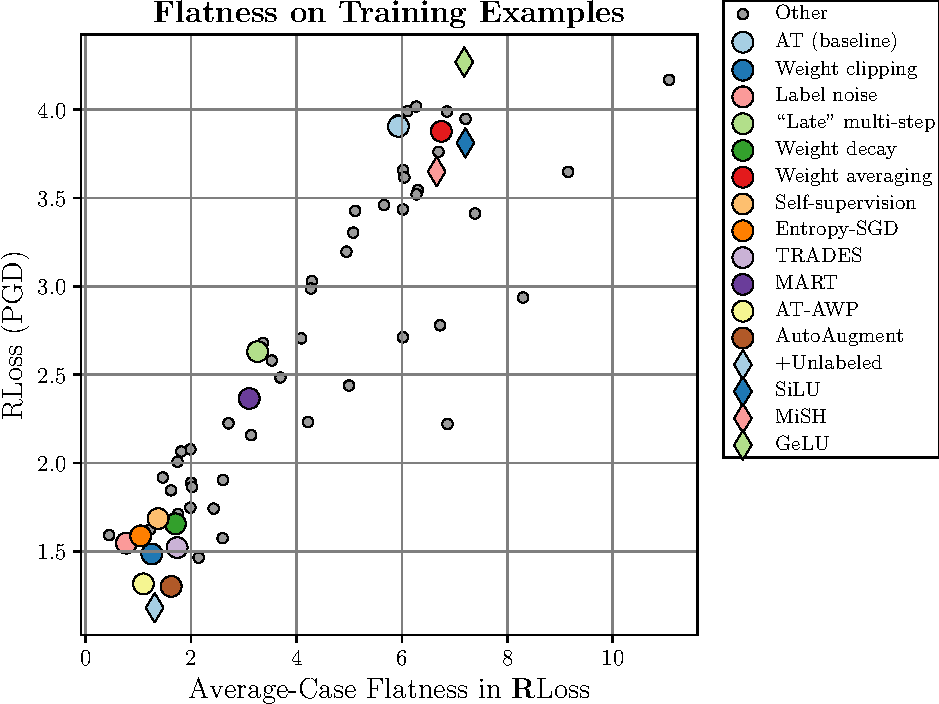
\includegraphics[height=3.6cm,clip,trim={0cm 0cm 3.75cm 0cm}]{plots_supp_flatness_correlation_seq_train_loss}
	\end{minipage}
	\hspace*{2px}
	\begin{minipage}[t]{0.2\textwidth}
		\vspace*{0px}
		
		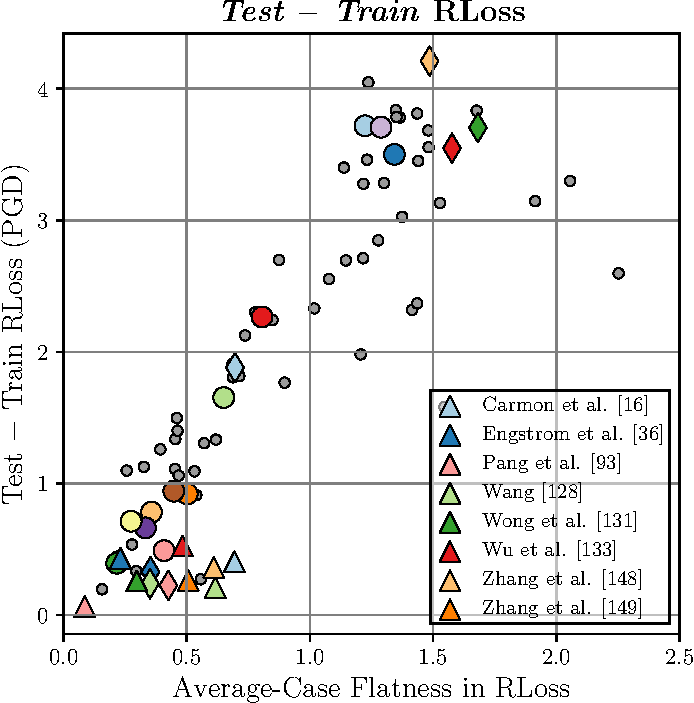
\includegraphics[height=3.6cm]{plots_main_flatness_seq_test_train_arxiv}
	\end{minipage}
	\hspace*{2px}
	\begin{minipage}[t]{0.27\textwidth}
		\vspace*{-2.5px}
		
		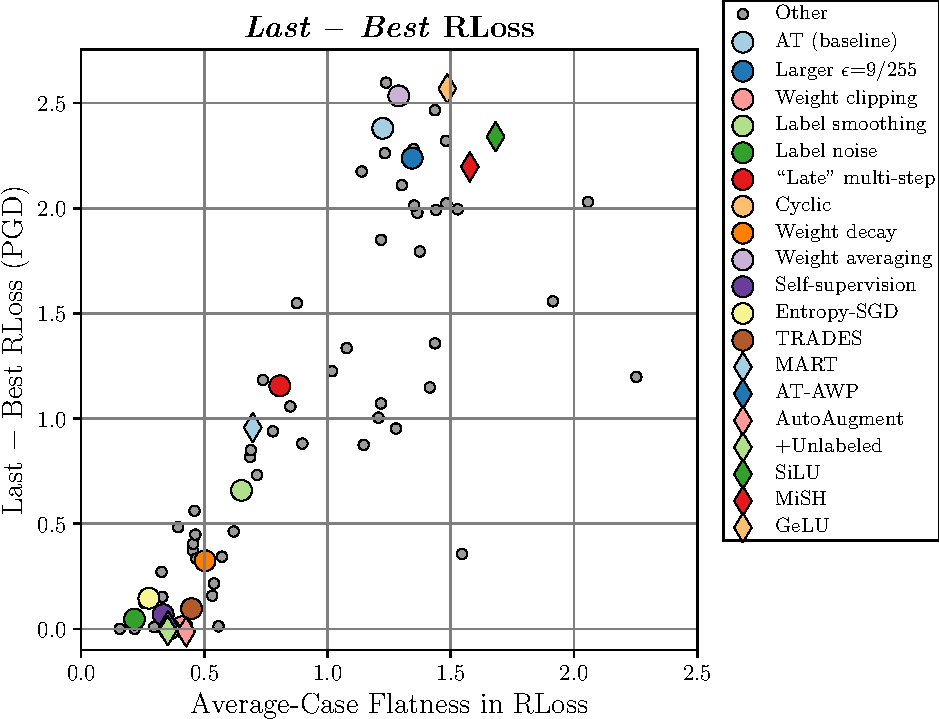
\includegraphics[height=3.7cm]{plots_main_flatness_correlation_seq_last_best_loss}
	\end{minipage}
	\hspace*{2px}
	\begin{minipage}[t]{0.01\textwidth}
		\vspace*{0px}
		
		\hspace*{4px}{\color{black!75}\rule{0.65px}{3.65cm}}
	\end{minipage}
	\hspace*{2px}
	\begin{minipage}[t]{0.265\textwidth}
		\vspace*{0px}
		
		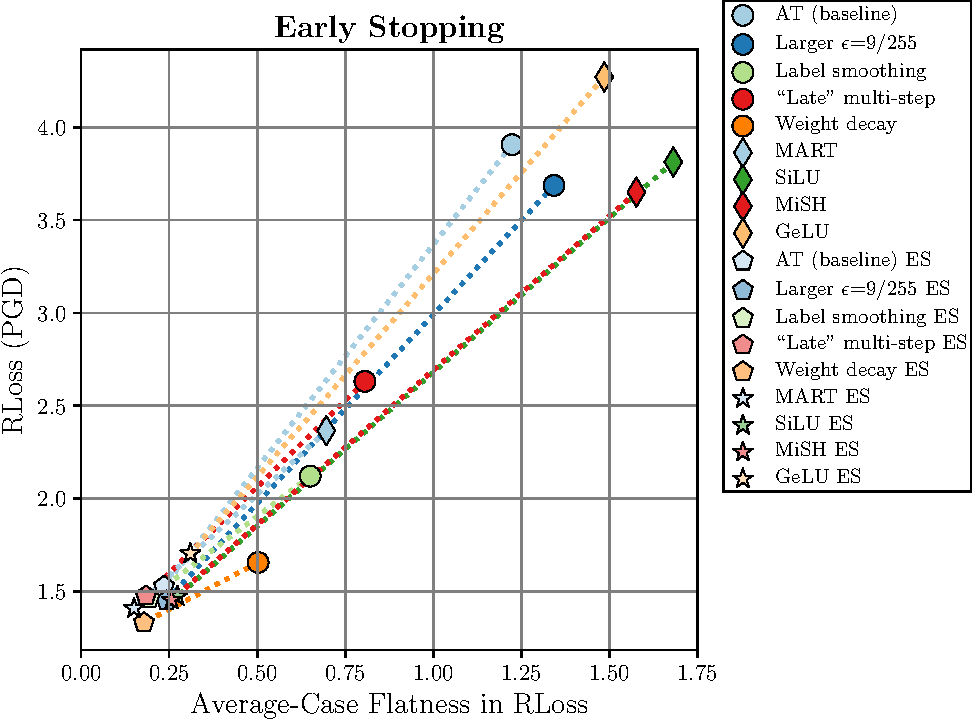
\includegraphics[height=3.6cm]{plots_main_flatness_correlation_seq_early_stopping_line}
	\end{minipage}	
	\vspace*{-8px}
	\caption{\textbf{Robust Generalization and Early Stopping.} \textbf{Left:} \red{\RCE plotted vs. average-case flatness measured \emph{on training examples}. Even on training examples, flatness is a good indicator for robust generalization.} \textbf{Middle:} Robust generalization (\RCE) decomposed into the test-train difference and the last-best (epoch) improvement (y-axis), both plotted against average-case flatness in \RCE(x-axis). In both cases, flatness seems to play an important role, \ie, flatness clearly reduces both the robust generalization gap \emph{and} robust overfitting. \textbf{Right:} \RCE vs\onedot average-case flatness in \RCE for selected models (all in supplementary material) with and without early stopping (``ES''). Early stopping consistently leads to improved adversarial robustness \emph{and} better flatness.}
	\label{fig:experiments-flatness-gap}
	\vspace*{-6px}
\end{figure*}

\subsection{Robust Generalization and Flatness in \RCE}
\label{subsec:experiments-flatness}

As robust overfitting is primarily avoided through strong regularization, we hypothesize that this is because strong regularization finds flatter minima in the \RCE landscape. These flat minima help to improve robust generalization.

\textbf{Flatness in \RCE ``Explains'' Overfitting:}
%
Using our average- and worst-case flatness measures in \RCE, we find that flatness reduces significantly during robust overfitting. Namely, flatness ``explains'' the increased \RCE caused by overfitting very well. \figref{fig:experiments-flatness-epochs} (left) plots \RCE, alongside average- and worst-case flatness and the maximum Hessian eigenvalue throughout training of our AT baseline. Clearly, flatness increases alongside (test) \RCE as soon as robust overfitting occurs. Note that the best epoch is $60$, meaning $0.4$ (black dotted). For further illustration, \figref{fig:experiments-flatness-epochs} (middle) explicitly plots \RCE (y-axis) against flatness in \RCE (x-axis) across epochs ({\color{blue!50!black}dark blue} to {\color{red!50!black}dark red}): \RCE and flatness clearly worsen ``alongside'' each other during overfitting, for both average- and worst-case flatness. Methods such as AT with self-supervision, AT-AWP or AT with unlabeled examples avoid both robust overfitting \emph{and} sharp minima (right).
This relationship generalizes to different hyper-parameter choices of these methods: \figref{fig:experiments-flatness-methods} plots \RCE (y-axis) vs\onedot average-case flatness (x-axis) across different hyper-parameters. Again, \eg, for {\color{plot9}TRADES} or {\color{plot10!80!black}AT-AWP}, hyper-parameters with lower \RCE also correspond to flatter minima.
In fact, \figref{fig:experiments-flatness-methods} indicates that the connection between robustness and flatness also generalizes \emph{across} different methods (and individual models).

\textbf{Improved Robustness Through Flatness:}
% 
Indeed, across all trained models, we found a \textbf{strong correlation between robust generalization and flatness}, using \RCE as measure for robust generalization.
As discussed in \secref{subsec:experiments-overfitting}, we mainly consider \RCE to assess robust generalization as improvements in \RCE above ${\sim}2.3$ have, on average, only small impact on \RTE. Pushing \RCE below $2.3$, in contrast, directly translates to better \RTE. This is illustrated in \figref{fig:experiments-flatness-correlation} (left) which plots \RTE vs\onedot \RCE for all evaluated models. To avoid this ``kink'' in the {\color{red}dotted red} lines around $\RCE{\approx}2.3$, \figref{fig:experiments-flatness-correlation} (middle left) plots \emph{\RCE} (y-axis) against \emph{average-case} flatness in \RCE (x-axis), highlighting selected models. This reveals a \emph{clear correlation between robustness and flatness}:
More robust methods, \eg, AT with unlabeled examples or AT-AWP, correspond to flatter minima. Methods improving flatness, \eg, Entropy-SGD, weight decay or weight clipping, improve adversarial robustness. This also translates to \RTE (middle right), subject to the described bend at $\RCE{\approx}2.3$. While many robust methods still obtain better flatness, activation functions such as SiLU, MiSH or GeLU also seem to improve flatness, without clear advantage in terms of robustness. Similarly, weight decay or clipping improve robustness considerably. \red{Overall, with Pearson/Spearman correlation coefficients of $0.85$/$0.87$ ($p$-values ${<}10^{-21}$), we revealed a strong relationship between robustness and flatness.}

\red{\figref{fig:experiments-flatness-correlation} (right) shows that this relationship is less clear when considering \emph{worst-case} flatness in \RCE (Pearson coefficient $0.54$). This is in contrast to \cite{WuNIPS2020} suggesting that worst-case flatness, in particular, is important to improve robustness of AT. However, worst-case flatness is more sensitive to $\xi$ and, thus, less comparable across methods. Note that worst-case robustness is still a good indicator for overfitting, \cf \figref{fig:experiments-flatness-epochs}.} All results are summarized in tabular form in \tabref{tab:experiments-flatness}: Grouping methods by \colorbox{colorbrewer3!15}{good}, \colorbox{colorbrewer5!15}{average} or \colorbox{colorbrewer1!15}{poor} robustness, we find that methods need at least ``some'' flatness, average- \emph{or} worst-case, to be successful.

\textbf{Decomposing Robust Generalization:}
%
So far, we used (absolute) \RCE on test examples as proxy of robust generalization. This is based on the assumption that deep models are generally able to obtain nearly zero \emph{train} \RCE. However, this is not the case for many methods in \tabref{tab:experiments-flatness} (second column). Thus, we also consider the robust generalization \emph{gap} and the \RCE difference between last and best (early stopped) epoch. \red{First, however, \figref{fig:experiments-flatness-gap} (left) shows that flatness, when measured on \emph{training examples}, is also a good predictor of (test) robustness.} Then, \figref{fig:experiments-flatness-gap} (middle left) explicitly plots the \RCE generalization gap (test$-$train \RCE, y-axis) against average-case flatness in \RCE (x-axis). Robust methods generally reduce this gap by \emph{both} reducing test \RCE \emph{and} avoiding convergence in train \RCE. Furthermore, \figref{fig:experiments-flatness-gap} (middle right) considers the difference between last and best epoch, essentially quantifying the extent of robust overfitting. Again, methods with small difference, \ie, little robust overfitting, generally correspond to flatter minima. This is also confirmed in \figref{fig:experiments-flatness-gap} (right) showing that early stopping essentially finds flatter minima along the training trajectory, thereby improving adversarial robustness.
Altogether, flatness improves robust generalization by reducing both the robust generalization gap \emph{and} the impact of robust overfitting.

\textbf{More Results:} \figref{fig:introduction} shows that the pre-trained models from RobustBench \cite{CroceARXIV2020b} confirm our observations so far (also see \figref{fig:experiments-flatness-gap}, middle left). While detailed analysis is not possible as only early stopped models are provided, they are consistently more robust \emph{and} correspond to flatter minima compared to our models. This is despite using different architectures (commonly Wide ResNets \cite{ZagoruykoBMVC2016}).